% ------------------------------------------------------------------------------
% Este fichero es parte de la plantilla LaTeX para la realización de Proyectos
% Final de Grado, protegido bajo los términos de la licencia GFDL.
% Para más información, la licencia completa viene incluida en el
% fichero fdl-1.3.tex

% Copyright (C) 2012 SPI-FM. Universidad de Cádiz
% ------------------------------------------------------------------------------

Para el diseño del sistema se ha optado por el patrón arquitectónico en tres capas. Éste divide el trabajo en tres niveles, repartiendo claramente las funciones.\\
Las capas se detallan a continuación:
\begin{itemize}
\item \textbf{Capa de presentación}: encargada de interactuar con el usuario.
\item \textbf{Capa de dominio}: encargada de implementar las funcionalidades del sistema.
\item \textbf{Capa de gestión de datos}: encargada de interactuar con el ``Sistema de Gestión de la Base de Datos (\textit{SGBD})''.
\end{itemize}
Las capas estan ordenadas de mayor a menor nivel de abstracción. Dichas capas se comunican con su capa contigua.\\

\section{Diseño de la capa de gestión de datos}
\subsection{Invocación de consultas SQL}
Las consultas SQL las realizan las clases declaradas en los archivos  principales ``.py'' de la aplicación.\\
\begin{itemize}
\item \textbf{La clase ``Dietista''}:
\begin{itemize}
\item \textbf{Método ``Verificar''}: realiza una consulta para verificar que un nuevo dietista no existe en el sistema.
\item \textbf{Método ``GuardarDietista''}: realiza una consulta para guardar los datos de un nuevo dietista en el sistema.
\item \textbf{Método ``MostrarDietistas''}: realiza una consulta para mostrar dietistas existentes en el sistema.
\item \textbf{Método ``Aceptar''}: realiza una consulta para verificar la contraseña de un dietista para su logueo en el sistema.
\item \textbf{Método ``ElimPerf''}: realiza una consulta para eliminar un dietista existente.
\end{itemize}
\item \textbf{La clase ``Paciente''}:
\begin{itemize}
\item \textbf{Método ``MostrarVentana2NPaciente''}: realiza una consulta para asignar un nuevo id al paciente nuevo.
\item \textbf{Método ``GuardarPaciente''}: realiza una consulta para guardar los datos de un paciente nuevo.
\item \textbf{Método ``AbrirPaciente''}: realiza una consulta para seleccionar los datos de un paciente existente.
\item \textbf{Método ``MostrarDatosP''}: realiza una consulta para mostrar todos los datos relacionados de un paciente existente.
\item \textbf{Método ``EliminarPaciente''}: realiza una consulta para tomar los datos del paciente a eliminar.
\item \textbf{Método ``DropPaciente''}: realiza una consulta para eliminar todos los datos relacionados del paciente.
\item \textbf{Método ``MostrarAnalisis''}: realiza una consulta para mostrar los análisis de un paciente.
\item \textbf{Método ``MostrarEnfPaciente''}: realiza una consulta para mostrar las enfermedades y patologías de un paciente.
\item \textbf{Método ``abrirDialogo''}: realiza una consulta para insertar un análisis a través de un diálogo de selección.
\item \textbf{Método ``EliminarAnalitica''}: realiza una consulta para eliminar una análisis.
\item \textbf{Método ``VerAnalitica''}: realiza una consulta para abrir el análisis.
\item \textbf{Método ``GuardarTrat''}: realiza una consulta para guardar el tratamiento farmacológico de un paciente.
\item \textbf{Método ``MostrarTratA''}: realiza una consulta para guardar el tratamiento de apoyo de un paciente.
\item \textbf{Método ``ElimItem''}: realiza una consulta para eliminar un tratamiento de apoyo de un paciente.
\item \textbf{Método ``ElimEnfBBDD''}: realiza una consulta para eliminar una enfermedad del sistema.
\item \textbf{Método ``CrearEnfermedad''}: realiza una consulta para crear una enfermedad o patología en el sistema.
\item \textbf{Método ``AnadirEnfermedad''}: realiza una consulta para añadir una enfermedad a un paciente.
\item \textbf{Método ``EliminarEP''}: realiza una consulta para eliminar una enfermedad del sistema.
\item \textbf{Método ``MostrarListadoEnf''}: realiza una consulta para mostrar el listado de enfermedades y patologías.
\item \textbf{Método ``ExcluirRecetasEnf''}: realiza una consulta para eliminar las recetas según los ingredientes que tenga la enfermedad.
\item \textbf{Método ``GuardarInfoG''}: realiza una consulta para guardar la información general de un paciente.
\item \textbf{Método ``MostrarInfoG''}: realiza una consulta para mostrar la información general de un paciente.
\item \textbf{Método ``MostrarDiario''}: realiza una consulta para mostrar los diarios dietéticos de un paciente.
\item \textbf{Método ``abrirDialogoD''}: realiza una consulta para añadir un diario dietético mediante un diálogo.
\item \textbf{Método ``EliminarDiario''}: realiza una consulta para eliminar un diario dietético seleccionado.
\item \textbf{Método ``VerDiario''}: realiza una consulta para abrir un diario dietético seleccionado.
\item \textbf{Método ``MostrarRecordatorio''}: realiza una consulta para mostrar los recordatorios 24h. existentes.
\item \textbf{Método ``abrirDialogoR''}: realiza una consulta para añadir un recordatorio 24h. mediante un diálogo.
\item \textbf{Método ``EliminarRecordatorio''}: realiza una consulta para eliminar un recordatorio 24h. seleccionado.
\item \textbf{Método ``VerRecordatorio''}: realiza una consulta para abrir un recordatorio 24h. seleccionado.
\item \textbf{Método ``MostrarPreferencias''}: realiza una consulta para iniciar la ventana de preferencias con los ingredientes existentes.
\item \textbf{Método ``AbrirCuestionarioFrec''}: realiza una consulta para abrir el cuestionario de frecuencia de un paciente.
\item \textbf{Método ``GuardarCuestionarioFrec''}: realiza una consulta para guardar el cuestionario de frecuencia del paciente.
\item \textbf{Método ``AccionGuardar''}: realiza una consulta para guardar los datos de un paciente.
\item \textbf{Método ``VerRecetas''}: realiza una consulta para mostrar los semanarios de un paciente.
\item \textbf{Método ``Ver''}: realiza una consulta para tomar los datos del semanario seleccionado.
\item \textbf{Método ``Utilizar''}: realiza una consulta para utilizar los datos en el semanario actual del semanario seleccionado. 
\item \textbf{Método ``Imprimir''}: realiza una consulta para tomar los datos a imprimir.
\end{itemize}
\item \textbf{La clase ``Receta''}:
\begin{itemize}
\item \textbf{Método ``MostrarIngred''}: realiza una consulta para mostrar todos los ingredientes existentes.
\item \textbf{Método ``AgregarIngr''}: realiza una consulta para agregar el ingrediente a la receta.
\item \textbf{Método ``ModificarIngr''}: realiza una consulta para modificar los datos de un ingrediente en la receta a modificar. 
\item \textbf{Método ``GuardarReceta''}: realiza una consulta para guardar los datos de la receta en el sistema.
\item \textbf{Método ``MostrarRecetas''}: realiza una consulta para mostrar la lista de recetas existentes.
\item \textbf{Método ``SeleccionarReceta''}: realiza una consulta para tomar los datos de una receta seleccionada.
\item \textbf{Método ``listElimReceta''}: realiza una consulta para mostrar las recetas existentes a eliminar.
\item \textbf{Método ``DropReceta''}: realiza una consulta para eliminar una receta.
\item \textbf{Método ``VentanaModificar''}: realiza una consulta para mostrar los datos de la receta a modificar.
\end{itemize}
\item \textbf{La clase ``Ingrediente''}:
\begin{itemize}
\item \textbf{Método ``GuardarIngrediente''}: realiza una consulta para guardar los datos de un ingrediente.
\item \textbf{Método ``ModificarIngrediente''}: realiza una consulta para modificar los datos de un ingrediente.
\item \textbf{Método ``RecogerPreferencias''}: realiza una consulta para mostrar las preferencias sobre el ingrediente.
\end{itemize}
\item \textbf{La clase ``Mainmenu''}:
\begin{itemize}
\item \textbf{Método ``mostrarPI''}: realiza una consulta para mostrar el peso ideal de un paciente.
\end{itemize}
\end{itemize}


\section{Diseño de la capa de dominio}
\subsection{Diagrama de interacción}
En este apartado se expondrán algunos de los diagramas de secuencia del diseño de la aplicación. Se utiliza un \textit{Patrón Controlador} en cada caso de uso descrito, es decir, una clase de control para llevar a cabo la operación solicitada.
\begin{itemize}
\item \textbf{Diagrama de secuencia para el caso de uso nuevo dietista}:
\begin{figure}[H]
  \label{ndiet}
  \begin{center}
    % Comentar si no está el paquete tkiz instalado, y descomentar la
    % linea siguiente. Comentar además la inclusión del paquete en
    % estilos/estiloBase.sty
    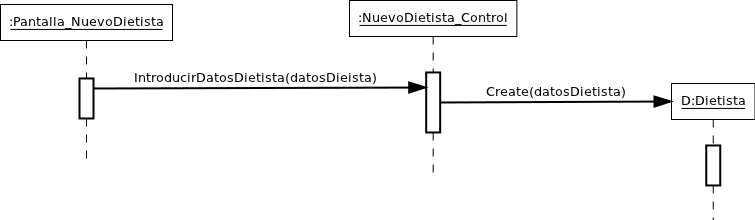
\includegraphics[scale=0.5]{../img/DI_NuevoDietista.png}
  \end{center}
  \caption{Diagrama de Interacción: Nuevo Dietista}
\end{figure}

\item \textbf{Diagrama de secuencia para el caso de uso nuevo paciente}: similar a aquellos casos de uso que suponen la creación de un objeto nuevo en la aplicación.
\begin{figure}[H]
  \label{npaciente}
  \begin{center}
    % Comentar si no está el paquete tkiz instalado, y descomentar la
    % linea siguiente. Comentar además la inclusión del paquete en
    % estilos/estiloBase.sty
    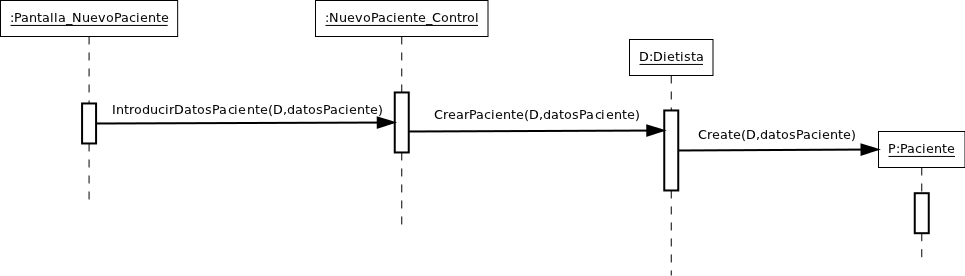
\includegraphics[scale=0.4]{../img/DI_NuevoPaciente.png}
  \end{center}
  \caption{Capa de presentación: Nuevo Paciente}
\end{figure}
\end{itemize}

A continuación se detallan los contratos de operaciones vistos en los diagramas de interacción.
\begin{itemize}
\item Nuevo Dietista:
\begin{itemize}
\item \textit{IntroducirDatosDietista(datosDietista)}: inicia la operación de introducción de los datos de un dietista en la aplicación.
\item \textit{Create(datosDietista)}: se crea un dietista con los datos especificados en datosDietista.
\end{itemize}
\item Nuevo Paciente:
\begin{itemize}
\item \textit{IntroducirDatosPaciente(D,datosPaciente)}: inicia la operación de introducción de los datos de un paciente en la aplicación.
\item \textit{CrearPaciente(D,datosPaciente)}: ordena al dietista D iniciar la creación de un paciente.
\item \textit{Create(D,datosPaciente)}: se crea un paciente con los datos especificados en datosPaciente.
\end{itemize}
\end{itemize}
\newpage


\section{Diseño de la capa de presentación}
Esta capa es la encargada de la interacción con el usuario, por lo que es importante que la primera impresión del usuario con respecto a la interfaz de la aplicación sea grata. La interfaz ha sido desarrollada bajo la biblioteca \textit{Qt}, así la apariencia visual de la misma se adaptará al tema de escritorio del usuario.\\
Se mostrarán a continuación algunos de los aspectos de la interfaz.
\begin{itemize}
\item \textbf{Menú principal}: ventana principal de la aplicación. Desde aquí el usuario podrá acceder a todas las funcionalidades del sistema. Se ha desarrollado buscando que la interfaz sea intuitiva, facilitando que el usuario encuentre rápidamente aquello que desee realizar. El menú principal constará de:
\begin{itemize}
\item \textbf{Barra de menú superior}: situado en la parte superior de la ventana, será la encargada de ofrecer las funcionalidades de los subsistemas de la aplicación. Cada botón tiene un nombre asociado referente a la tarea que realiza, facilitando así la interactuación del usuario.
\item \textbf{Área de información rápida}: situado inmediatamente debajo de la barra de menú superior, será donde el dietista podrá visualizar las referencias rápidas de ese paciente como recordatorio y orientación, facilitando así el trabajo.
\item \textbf{Pestañas interiores de información e interactuación}: a continuación nos encontramos con las pestañas de información e interactuación, desde las cuales el dietista podrá consultar y modificar los datos de un paciente, clasificados en pestañas que engloban información relacionada, haciendo más intuitivo el trabajo.
\begin{figure}[H]
  \label{ppral}
  \begin{center}
    % Comentar si no está el paquete tkiz instalado, y descomentar la
    % linea siguiente. Comentar además la inclusión del paquete en
    % estilos/estiloBase.sty
    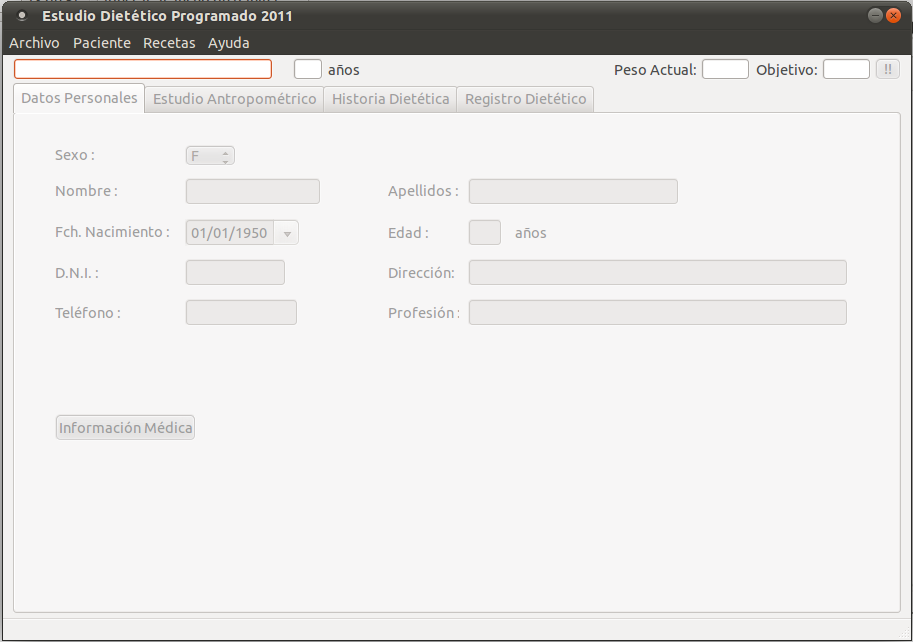
\includegraphics[scale=0.5]{../../Image/aplicacion.png}
  \end{center}
  \caption{Capa de presentación: Menú Principal}
\end{figure}
\end{itemize}

\newpage
\item \textbf{Pestañas de información e interactuación:} constará de cuatro pestañas, desde las cuales se manejará la información relevante sobre el paciente.
\begin{itemize}
\item \textbf{Datos Personales}: ubicación de los datos personales más relevantes del paciente, a los que el dietista puede recurrir de un vistazo.\\\\
\begin{figure}[H]
  \label{datos}
  \begin{center}
    % Comentar si no está el paquete tkiz instalado, y descomentar la
    % linea siguiente. Comentar además la inclusión del paquete en
    % estilos/estiloBase.sty
    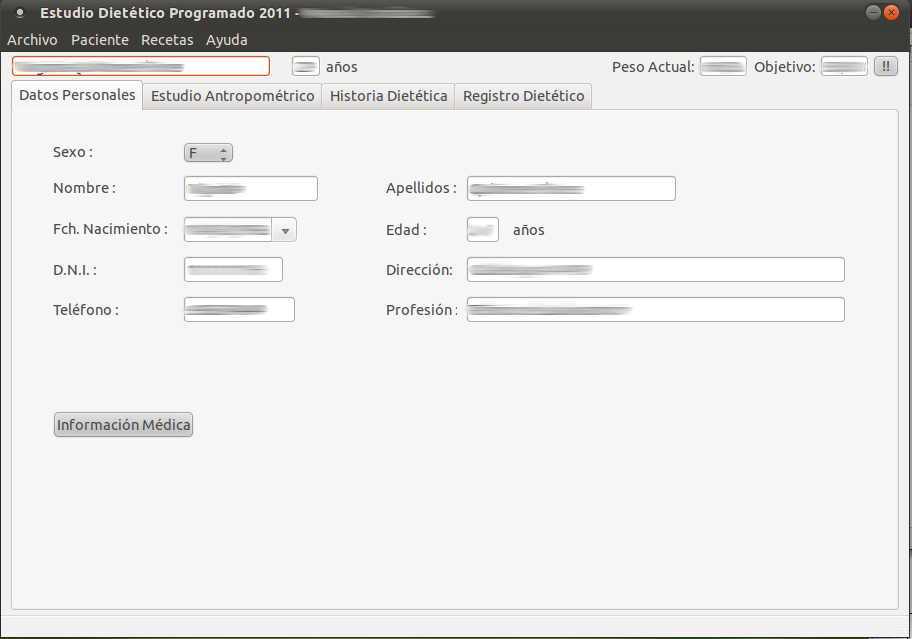
\includegraphics[scale=0.5]{../../Image/paciente-datos.png}
  \end{center}
  \caption{Capa de presentación: Pestaña Datos Personales}
\end{figure}
\newpage
\item \textbf{Estudio Antropométrico}: ubicación de los datos antropométricos del paciente, desde el cual se trabajará en mayor medida a lo largo del seguimiento del paciente.\\\\
\begin{figure}[H]
  \label{antrop}
  \begin{center}
    % Comentar si no está el paquete tkiz instalado, y descomentar la
    % linea siguiente. Comentar además la inclusión del paquete en
    % estilos/estiloBase.sty
    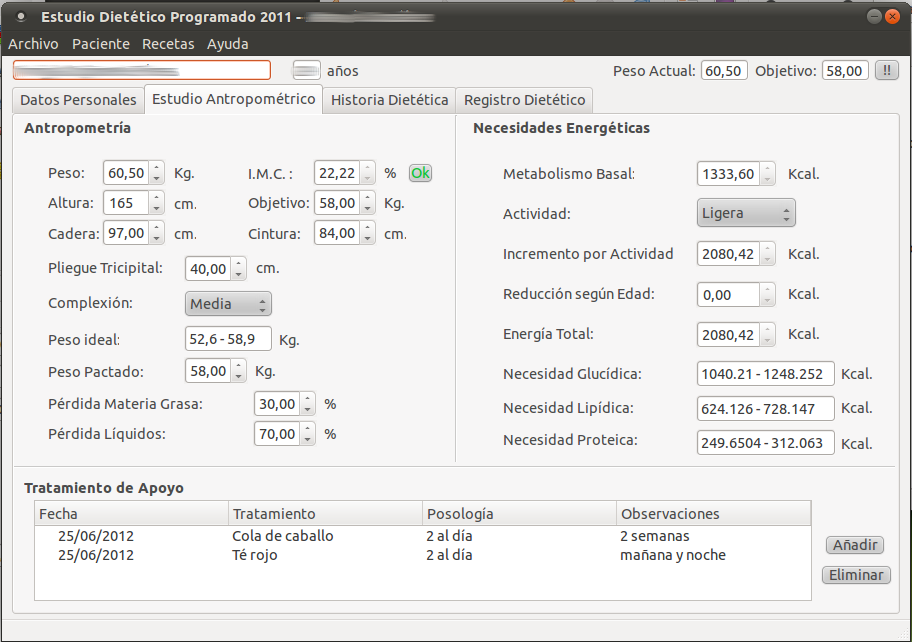
\includegraphics[scale=0.5]{../../Image/paciente-antrop.png}
  \end{center}
  \caption{Capa de presentación: Pestaña Estudio Antropométrico}
\end{figure}
\newpage
\item \textbf{Historia Dietética}: desde aquí se podrá acceder a otras ventanas que tendrán como propósito albergar otros datos menos recurrentes pero necesarios acerca del paciente.\\\\
\begin{figure}[H]
  \label{hist}
  \begin{center}
    % Comentar si no está el paquete tkiz instalado, y descomentar la
    % linea siguiente. Comentar además la inclusión del paquete en
    % estilos/estiloBase.sty
    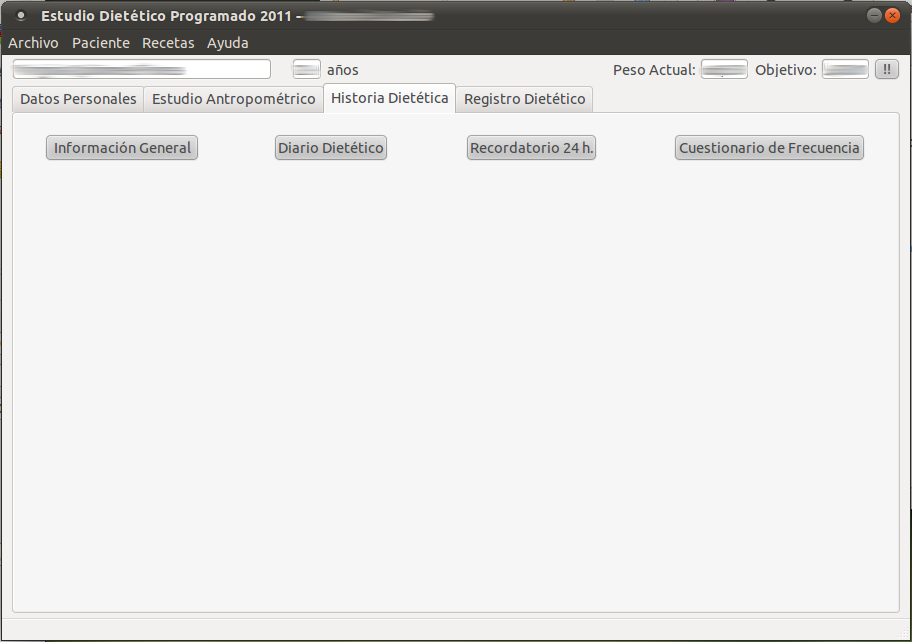
\includegraphics[scale=0.5]{../../Image/paciente-hist.png}
  \end{center}
  \caption{Capa de presentación: Pestaña Historia Dietética}
\end{figure}
\newpage
\item \textbf{Registro Dietético}: desde aquí se realizarán los semanarios que sirven de guía al paciente y le enseña a tener una buena alimentación, el cual es el mayor propósito de la aplicación.\\\\
\begin{figure}[H]
  \label{registro}
  \begin{center}
    % Comentar si no está el paquete tkiz instalado, y descomentar la
    % linea siguiente. Comentar además la inclusión del paquete en
    % estilos/estiloBase.sty
    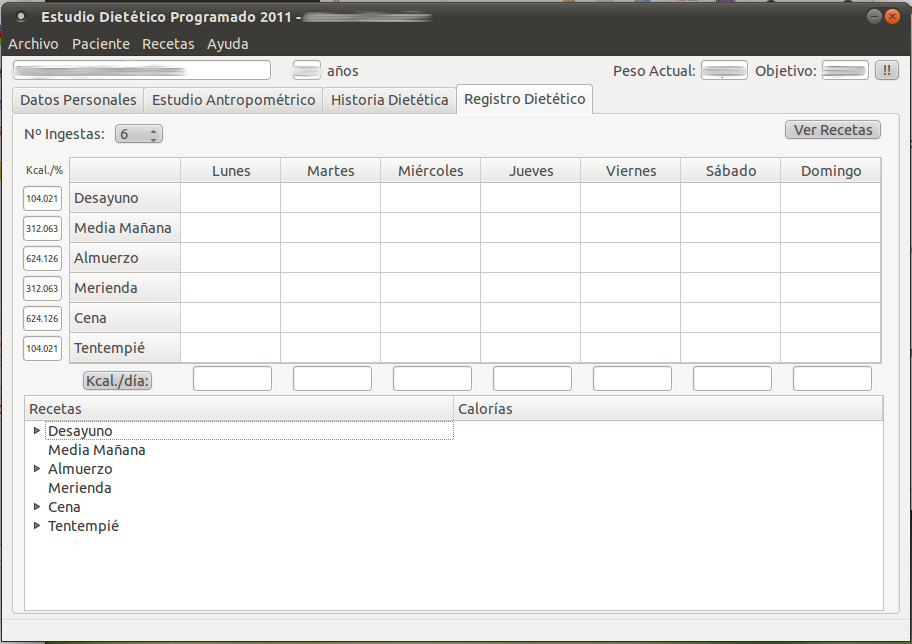
\includegraphics[scale=0.5]{../../Image/paciente-registro.png}
  \end{center}
  \caption{Capa de presentación: Pestaña Registro Dietético}
\end{figure}
\end{itemize}
\newpage
\item \textbf{Formularios de registro}: formulario para introducir datos en el sistema, en este caso, para el alta de un paciente. Se compone de los siguientes elementos:
\begin{itemize}
\item \textbf{Etiquetas identificativas}: indican el dato a introducir.
\item \textbf{Campo de texto}: donde el dietista introduce los datos.
\item \textbf{Botones de opción}: albergando los botones aceptar, que guardará los datos y el botón cancelar, que cancela el proceso.
\end{itemize}
\begin{figure}[H]
  \label{pnuevo}
  \begin{center}
    % Comentar si no está el paquete tkiz instalado, y descomentar la
    % linea siguiente. Comentar además la inclusión del paquete en
    % estilos/estiloBase.sty
    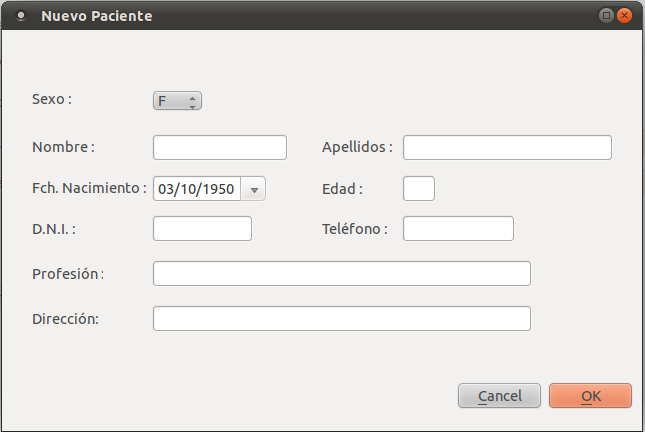
\includegraphics[scale=0.5]{../../Image/paciente-nuevo1.png}
  \end{center}
  \caption{Capa de presentación: Formulario Nuevo Paciente}
\end{figure}

\item \textbf{Nueva Receta}: formulario asociado al alta de una nueva receta. Éste cuenta con campos distintos al anterior, que se detallan a continuación:
\begin{itemize}
\item \textbf{Etiquetas identificativas}: indican el dato a introducir.
\item \textbf{Campos de texto}: donde el dietista introduce los datos.
\item \textbf{Selección de ingredientes}: selección de los ingredientes que forman parte de la receta.
\item \textbf{Desplegable de selección}: desplegable de categoría de receta.
\end{itemize}
\begin{figure}[H]
  \label{nreceta}
  \begin{center}
    % Comentar si no está el paquete tkiz instalado, y descomentar la
    % linea siguiente. Comentar además la inclusión del paquete en
    % estilos/estiloBase.sty
    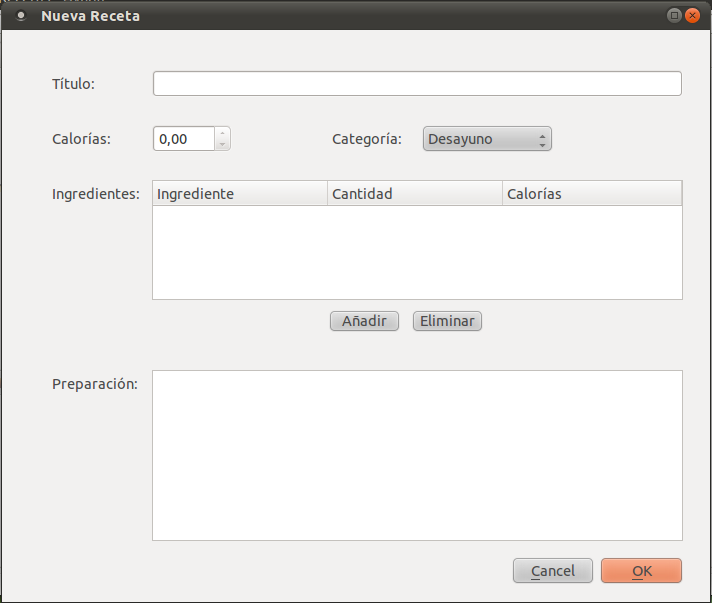
\includegraphics[scale=0.5]{../../Image/receta-nueva.png}
  \end{center}
  \caption{Capa de presentación: Formulario Nueva Receta}
\end{figure}
\end{itemize}

\section{Diseño de la base de datos}
\subsection{Diseño conceptual de la base de datos}
\begin{itemize}
\item Tipos de entidades:\\\\
A continuación se exponen las distintas entidades que intervendrán en la aplicación, así como los atributos que poseen cada una de ellas. \\
\begin{table}[H]
\begin{center}
  \begin{tabular}{| l | p{12cm} |}
    \hline
    Entidad & Atributos \\ \hline
    Dietista & Dni, Nombre, Password \\ \hline
    Paciente & Id\_paciente, Sexo, Dni, Nombre, Apellidos, Fch\_Nac, Tlf, Profesion, Direccion \\ \hline
	Antrop\_Nec & Id\_antropnec, Peso, Altura, Imc, Objetivo, Cadera, Cintura, Plieguetric, Complexion, Pesopactado, Mb, Actividad, EnergiaTotal, NumIngesta, PerdidaMatGrasa, InformacionTrat \\ \hline
	Analisis & Id\_analisis, Ruta, Nombre, Fecha \\ \hline
	Diario\_Dietetico & Id\_diario, Ruta, Nombre, Fecha \\ \hline
	Recordatorio & Id\_recordatorio, Ruta, Nombre, Fecha \\ \hline
	Info\_Gen & Id\_ig, camporegistro, contenidoregistro \\ \hline
	Trat\_Apoyo & Id\_tratapoyo, Fecha, Tratamiento, Psologia, Observaciones \\ \hline
	Peso\_Ideal & Id\_pesoideal, Fm, Complexion, Altura, Peso \\ \hline
	Receta & Id\_receta, Nombre, Calorias, Categoria, Preparacion \\ \hline
	Ingrediente & Id\_ingrediente, Nombre, Cantidad, Tipo, Calorias \\ \hline
	Enfermedad & Id\_enfermedad, Nombre \\ \hline
	Semanario & Id\_semanario, Lunes, Martes, Miercoles, Jueves, Viernes, Sabado, Domingo, kcal\_dia, Fecha, Kcalorias, Numingestas \\
	\hline
  \end{tabular}
\end{center}
\caption{Tabla de entidades}
\end{table}
\item Tipo de relaciones:\\\\
Las relaciones intervinientes son:
\begin{itemize}
\item \textbf{Pertenece a}: Relación que existe entre los dietistas y los pacientes.
\item \textbf{Posee}: Relación que existe entre los pacientes y los semanarios.
\item \textbf{Pacede}: Relación que existe entre los pacientes y las enfermedades.
\item \textbf{Tiene}: Relación que existe entre los semanarios y las recetas.
\item \textbf{Es autor de}: Relación que existe entre los dietistas y las recetas.
\item \textbf{Prohibe}: Relación que existe entre las enfermedades y los ingredientes.
\item \textbf{Necesita}: Relación que existe entre los ingredientes y las recetas.
\item \textbf{Es su}: Relación que existe entre los pesos ideales y los pacientes.
\item \textbf{Le corresponde}: Relación que existe entre las necesidades antropométricas y los pacientes.
\item \textbf{Realiza}: Relación que existe entre los diarios dietéticos y los pacientes.
\item \textbf{Recuerda}: Relación que existe entre los recordatorios y los pacientes.
\item \textbf{Se hace}: Relación que existe entre los análisis y los pacientes.
\item \textbf{Prefiere}: Relación que existe entre los ingredientes y los pacientes.
\item \textbf{Informa}: Relación que existe entre las informaciones generales y los pacientes.
\item \textbf{Toma}: Relación que existe entre los tratamientos de apoyo y los pacientes.
\end{itemize}

\newpage
\item Diagrama Entidad-Relación:\\
Para mayor comprensión del diagrama se omiten los atributos proporcionados en la tabla de entidades.
\begin{figure}[H]
  \label{d_er}
  \begin{center}
    % Comentar si no está el paquete tkiz instalado, y descomentar la
    % linea siguiente. Comentar además la inclusión del paquete en
    % estilos/estiloBase.sty
    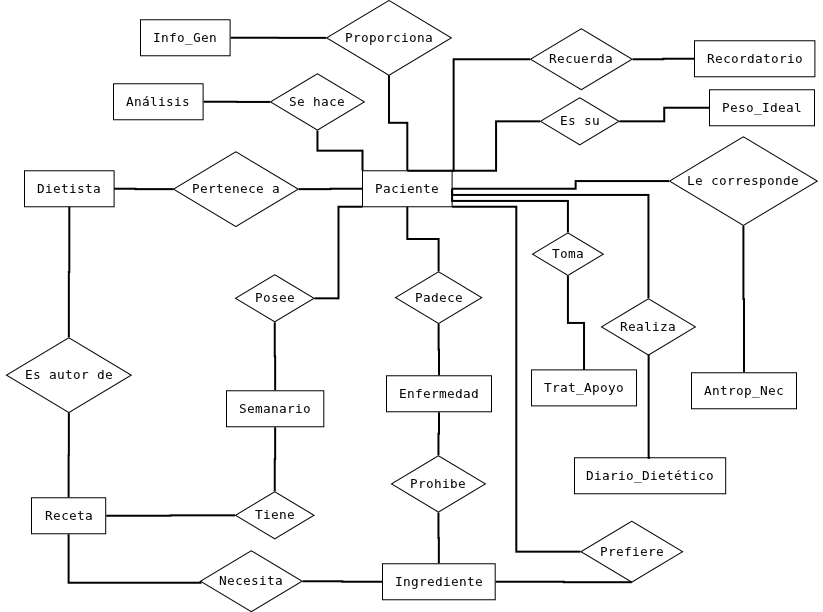
\includegraphics[scale=0.6]{../img/Diagrama_ER.png}
  \end{center}
  \caption{Diagrama Entidad Relación}
\end{figure}
\end{itemize}
\newpage
\subsection{Diseño lógico de la base de datos}
Después de realizar el estudio lógico de la base de datos, las tablas resultantes son:
\begin{itemize}
\item \textbf{Dietista}: (Dni, Nombre, Password)
\begin{itemize}
\item Clave primaria: \textit{Dni}
\item Se incluye \textit{Dni} en las tablas ``Paciente'', ``Receta'' y ``Receta\_Ingredientes''
\end{itemize}
\item \textbf{Paciente}: (Id\_paciente, Sexo, Dni, Nombre, Apellidos, Fch\_Nac, Tlf, Profesion, Direccion, Dni\_Diet)
\begin{itemize}
\item Clave primaria: \textit{Id\_paciente}
\item Clave foránea: \textit{Dni\_Diet}
\item Se incluye \textit{Id\_paciente} en las tablas ``Análisis'', ``Antrop\_Nec'', ``Diario\_Diet'', ``Enf\_Paciente'', ``Info\_gen'', ``Recordatorio'', ``Preferencia'', ``Semanario'' y ``Trat\_Apoyo''
\end{itemize}
\item \textbf{Antrop\_Nec}: (Id\_antropnec, Peso, Altura, Imc, Objetivo, Cadera, Cintura, Plieguetric, Complexion, Pesopactado, Mb, Actividad, EnegiaTotal, NumIngesta, PerdidaMatGrasa, InformacionTrat, Id\_paciente)
\begin{itemize}
\item Clave primaria: \textit{Id\_antropnec}
\item Clave foránea: \textit{Id\_paciente}
\end{itemize}
\item \textbf{Analisis}: (Id\_analisis, Ruta, Nombre, Fecha, Id\_paciente)
\begin{itemize}
\item Clave primaria: \textit{Id\_analisis}
\item Clave foránea: \textit{Id\_paciente}
\end{itemize}
\item \textbf{Diario\_Dietetico}: (Id\_diario, Ruta, Nombre, Fecha, Id\_paciente)
\begin{itemize}
\item Clave primaria: \textit{Id\_diario}
\item Clave foránea: \textit{Id\_paciente}
\end{itemize}
\item \textbf{Recordatorio}: (Id\_recordatorio, Ruta, Nombre, Fecha, Id\_paciente)
\begin{itemize}
\item Clave primaria: \textit{Id\_recordatorio}
\item Clave foránea: \textit{Id\_paciente}
\end{itemize}
\item \textbf{Info\_Gen}: (Id\_ig, camporegistro, contenidoregistro, Id\_paciente)
\begin{itemize}
\item Clave primaria: \textit{Id\_ig}
\item Clave foránea: \textit{Id\_paciente}
\end{itemize}
\item \textbf{Trat\_Apoyo}: (Id\_tratapoyo, Fecha, Tratamiento, Psologia, Observaciones, Id\_paciente)
\begin{itemize}
\item Clave primaria: \textit{Id\_tratapoyo}
\item Clave foránea: \textit{Id\_paciente}
\end{itemize}
\item \textbf{Peso\_Ideal}: (Id\_pesoideal, Fm, Complexion, Altura, Peso, Id\_paciente)
\begin{itemize}
\item Clave primaria: \textit{Id\_pesoideal}
\item Clave foránea: \textit{Id\_paciente}
\end{itemize}
\item \textbf{Receta}: (Id\_receta, Nombre, Calorias, Categoria, Preparacion, Dni\_Diet)
\begin{itemize}
\item Clave primaria: \textit{Id\_receta}
\item Clave foránea: \textit{Dni\_Diet}
\item Se incluye \textit{Nombre} en la tabla ``Receta\_Ingredientes''
\end{itemize}
\item \textbf{Ingrediente}: (Id\_ingrediente, Nombre, Cantidad, Tipo, Calorias)
\begin{itemize}
\item Clave primaria: \textit{Id\_ingrediente}
\item Se incluye \textit{Id\_Ingrediente} en la tabla ``Enf\_Ingred'', se incluye \textit{Nombre} en la tabla ``Receta\_Ingredientes''
\end{itemize}
\item \textbf{Receta\_Ingredientes}: (Id\_recing, NombreRec, NombreIngred, CantIngred, CalIngred, Dni\_Diet)
\begin{itemize}
\item Clave primaria: \textit{Id\_recing}
\item Clave foránea: \textit{Dni\_Diet}, \textit{NombreRec}, \textit{NombreIngred}
\end{itemize}
\item \textbf{Enfermedad}: (Id\_enfermedad, Nombre)
\begin{itemize}
\item Clave primaria: \textit{Id\_enfermedad}
\item Se incluye \textit{Id\_enfermedad} en las tablas ``Enf\_Ingred'' y ``Enf\_Paciente''
\end{itemize}
\item \textbf{Enf\_Ingred}: (Id\_enfingred, Id\_enfermedad, Id\_ingrediente)
\begin{itemize}
\item Clave primaria: \textit{Id\_enfingred}
\item Clave foránea: \textit{Id\_enfermedad} e \textit{Id\_ingrediente}
\end{itemize}
\item \textbf{Enf\_Paciente}: (Id\_enfpac, Id\_paciente, Id\_enfermedad)
\begin{itemize}
\item Clave primaria: \textit{Id\_enfpac}
\item Clave foránea: \textit{Id\_enfermedad} e \textit{Id\_paciente}
\end{itemize}
\item \textbf{Semanario}: (Id\_semanario, Lunes, Martes, Miercoles, Jueves, Viernes, Sabado, Domingo, kcal\_dia, Fecha, Kcalorias, Numingestas, Id\_paciente)
\begin{itemize}
\item Clave primaria: \textit{Id\_semanario}
\item Clave foránea: \textit{Id\_paciente}
\end{itemize}
\end{itemize}
Una vez obtenidas las tablas, se va a proceder a la normalización.\\
La normalización de la base de datos es una serie de reglas que permiten a los diseñadores de bases de datos desarrollar un esquema que minimice los problemas de lógica.\\
Una base de datos normalizada ofrece mayor comprensión de la misma y ocupa un espacio menor debido a la menor repetición de datos.\\\\
En nuestra base de datos se van a aplicar 3 grados de normalización, los cuales son:
\begin{itemize}
\item \textbf{1ª Forma Normal}: establece que todos los atributos de la tabla deben ser atómicos (indivisibles),
existe una clave primaria con atributos y estos son no nulos. Con esto se consiguen eliminar los valores repetidos en una base de datos.
\item \textbf{2ª Forma Normal}: establece que aquellos datos que no dependen de la clave primaria se deben eliminar y separar dentro de sus propias tablas.
\item \textbf{3ª Forma Normal}: una tabla esta en 3ª Forma Normal si todos los datos son dependientes funcionalmente de la clave primaria y no existe dependencias transitivas, es decir, que una columna dependa de otra y ninguna de ellas sea clave primaria.
\end{itemize}

A continuación se aplicarán los 3 grados de normalización a las tablas obtenidas previamente:

\begin{itemize}
\item \textbf{1ª Forma Normal}: todas las tablas se encuentran en 1ª Forma Normal, porque todos sus atributos son atómicos, y tienen una única clave primaria no nula.
\item \textbf{2ª Forma Normal}: todas las tablas se encuentran en 2ª Forma Normal, puesto que estan en 1ª Forma Normal y su clave primaria es un único atributo.
\item \textbf{3ª Forma Normal}: en este caso, en la tabla ``Antrop\_Nec'' observamos que el campo ``Imc'' depende de los campos ``Peso'' y ``Altura'', así mismo el campo ``Mb'' depende de los campos ``Objetivo'' y ``Complexion'', y también se observa que el campo ``EnergiaTotal'' depende de los campos ``Mb'' y ``Actividad''.
Para solucionar el problema podríamos dividir la tabla de modo que cumpliera la 3ª Forma Normal, tal que así:

\begin{table}[H]
\begin{center}
  \begin{tabular}{| l | p{8cm} |}
    \hline
    Entidad & Atributos \\ \hline
	Antrop\_Nec & Id\_antropnec, Peso, Altura, Objetivo, Cadera, Cintura, Plieguetric, Complexion, Pesopactado, Actividad, NumIngesta, PerdidaMatGrasa, InformacionTrat \\ \hline
	Imc\_Paciente & Id\_imc, Imc, Id\_antropnec \\ \hline
	Mb\_Paciente & Id\_mb, Mb, Id\_antropnec \\ \hline
	ET\_Paciente & Id\_et, EnergiaTotal, Id\_antropnec \\
	\hline
  \end{tabular}
\end{center}
\caption{Normalización 3º Forma Normal}
\end{table}
\end{itemize}

A continuación se muestran las tablas después del proceso de normalización. Para mayor comprensión las claves primarias aparecen subrayadas y las claves foráneas aparecen en cursiva.

\begin{table}[H]
\begin{center}
  \begin{tabular}{| l | p{12cm} |}
    \hline
    Entidad & Atributos \\ \hline
    Dietista & \underline{Dni}, Nombre, Password \\ \hline
    Paciente & \underline{Id\_paciente},  Sexo, Dni, Nombre, Apellidos, Fch\_Nac, Tlf, Profesion, Direccion, \textit{Dni\_Diet} \\ \hline
	Antrop\_Nec & \underline{Id\_antropnec}, Peso, Altura, Objetivo, Cadera, Cintura, Plieguetric, Complexion, Pesopactado, Actividad, NumIngesta, PerdidaMatGrasa, InformacionTrat, \textit{Id\_paciente} \\ \hline
	Imc\_Paciente & \underline{Id\_imc}, Imc, \textit{Id\_antropnec} \\ \hline
	Mb\_Paciente & \underline{Id\_mb}, Mb, \textit{Id\_antropnec} \\ \hline
	ET\_Paciente & \underline{Id\_et}, EnergiaTotal, \textit{Id\_antropnec} \\ \hline
	Analisis & \underline{Id\_analisis}, Ruta, Nombre, Fecha, \textit{Id\_paciente} \\ \hline
	Diario\_Dietetico & \underline{Id\_diario}, Ruta, Nombre, Fecha, \textit{Id\_paciente} \\ \hline
	Recordatorio & \underline{Id\_recordatorio}, Ruta, Nombre, Fecha, \textit{Id\_paciente} \\ \hline
	Info\_Gen & \underline{Id\_ig}, camporegistro, contenidoregistro, \textit{Id\_paciente} \\ \hline
	Trat\_Apoyo & \underline{Id\_tratapoyo}, Fecha, Tratamiento, Psologia, Observaciones, \textit{Id\_paciente} \\ \hline
	Peso\_Ideal & \underline{Id\_pesoideal}, Fm, Complexion, Altura, Peso, \textit{Id\_paciente} \\ \hline
	Receta & \underline{Id\_receta}, Nombre, Calorias, Categoria, Preparacion, \textit{Dni\_Diet} \\ \hline
	Ingrediente & \underline{Id\_ingrediente}, Nombre, Cantidad, Tipo, Calorias \\ \hline
	Receta\_Ingredientes & \underline{Id\_recing}, NombreRec, NombreIngred, CantIngred, CalIngred, \textit{Dni\_Diet} \\ \hline
	Enfermedad & \underline{Id\_enfermedad}, Nombre \\ \hline
	Enf\_Ingred & \underline{Id\_enfingred}, \textit{Id\_enfermedad}, \textit{Id\_ingrediente} \\ \hline
	Enf\_Paciente & \underline{Id\_enfpac}, \textit{Id\_paciente}, \textit{Id\_enfermedad} \\ \hline
	Semanario & \underline{Id\_semanario}, Lunes, Martes, Miercoles, Jueves, Viernes, Sabado, Domingo, kcal\_dia, Fecha, Kcalorias, Numingestas, \textit{Id\_paciente} \\
	\hline
  \end{tabular}
\end{center}
\caption{Tablas normalizadas}
\end{table}

\subsection{Diseño físico de la base de datos}
Una vez tenemos las tablas normalizadas con las que trabajaremos pasamos a la implementación de las mismas.
Observamos que durante la normalización creamos tablas nuevas, llamadas ``Imc\_Paciente'', ``Mb\_Paciente'' y ``ET\_Paciente'', pero realmente no optimizan el diseño ni la comprensión de las tablas.\\
Por tanto desnormalizaremos dichas tablas volviendo a incluir los respectivos campos en las tablas de las que provenían, ``Antrop\_Nec'', eliminando así las tablas ``Imc\_Paciente'', ``Mb\_Paciente'' y ``ET\_Paciente''.

\begin{table}[H]
\begin{center}
  \begin{tabular}{| l | p{12cm} |}
    \hline
    Entidad & Atributos \\ \hline
    Antrop\_Nec & \underline{Id\_antropnec}, Peso, Altura, Imc, Objetivo, Cadera, Cintura, Plieguetric, Complexion, Pesopactado, Mb, Actividad, EnergiaTotal, NumIngesta, PerdidaMatGrasa, InformacionTrat, \textit{Id\_paciente} \\ 
	\hline
  \end{tabular}
\end{center}
\caption{Tabla ``Antrop\_Nec'' desnormalizada}
\end{table}

\newpage

%
%\section{Diseño de la arquitectura}
%En esta sección se define la arquitectura general del sistema de información, especificando las distintas particiones físicas del mismo, la descomposición lógica en subsistemas de diseño y la ubicación de cada subsistema en cada partición, así como la especificación detallada de la infraestructura tecnológica necesaria para dar soporte al sistema de información.
%
%\subsection{Arquitectura física}
%En este apartado, describimos los principales componentes hardware que forman la arquitectura física de nuestro sistema, recogiendo por un lado los componentes de servidor y los componentes de sistemas externos con los que colabora nuestro sistema y por otro, los componentes hardware de cliente.
%
%\subsection{Arquitectura lógica}
%La arquitectura lógica del sistema está formada por los elementos software (servicios, aplicaciones, librerías, frameworks, etc.) que componen el software base, más el software desarrollado para cumplir los requisitos de la aplicación. También, se recogen los componentes de sistemas externos con los que interactúa nuestro sistema, así como los componentes software del lado cliente.
%
%\subsection{Arquitectura de diseño}
%La arquitectura de diseño especifica la forma en que los artefactos software de más bajo nivel, interactúan entre sí para lograr el comportamiento deseado en el sistema. Utilizaremos el patrón arquitectónico  Layers (Capas), con el cual estructuramos el sistema en un número apropiado de capas, de forma que todos los componentes de una misma capa trabajan en el mismo nivel de abstracción y los servicios proporcionados por la capa superior utilizan internamente los servicios proporcionados por la capa inmediatamente inferior.
%
%\subsubsection{Capa de presentación}
%Este grupo de artefactos software conforman la capa de presentación del sistema, incluyendo tanto los componentes de la vista como los elementos de control de la misma.
%\subsubsection{Capa de negocio}
%Este grupo de artefactos software conforman la capa de negocio del sistema, incluyendo los elementos del modelo de dominio y los servicios (operaciones del sistema).
%\subsubsection{Capa de integración}
%Este grupo de artefactos software conforman la capa de integración del sistema, incluyendo las clases de abstracción para el acceso a datos (BD o sistema de ficheros) o a sistemas heredados.
%\subsubsection{Servicios transversales}
%Este grupo de artefactos software pueden ser usados por elementos de cualquiera de las capas del sistema y fundamentalmente proporcionan servicios relacionados con requisitos no funcionales (calidad).
%
%
%\section{Diseño de la interfaz de usuario} 
%En esta sección se especifican las interfaces entre el sistema y el usuario, detallando el aspecto y el comportamiento de las diferentes pantallas e informes, de acuerdo con el entorno tecnológico definido. Con respecto a las pantallas e informes, es preciso realizar un prototipo o mockup gráfico. Junto a estos bocetos hay que definir qué ocurre en los distintos componentes visuales de la interfaz cuando aparecen y qué acciones se disparan cuando el usuario trabaja con ellas.
%Además, es preciso elaborar un diagrama de navegación, reflejando la secuencia de pantallas a las que tienen acceso los diferentes roles de usuario y la conexión entre éstas. 
%
%
%\section{Diseño de datos}
%En esta sección se define la estructura física de datos que utilizará el sistema, a partir del modelo de conceptual de clases, de manera que teniendo presente los requisitos establecidos para el sistema de información y las particularidades del entorno tecnológico, se consiga un acceso eficiente de los datos. La estructura física se compone de tablas, índices, procedimientos almacenados, secuencias y otros elementos dependientes del SGBD a utilizar.
%
%
%\section{Diseño de componentes}
%En esta sección se definen los componentes software necesarios para la implementación del sistema. Para facilitar la comprensión y la posterior implementación del sistema, es recomendable organizarlo en forma de subsistemas, los cuales se compondrán a su vez de módulos. Estos módulos (o paquetes) contendrán un conjunto de artefactos software, que representaremos en forma de clases y que corresponderán a una de las capas identificadas en la arquitectura. 
%Para cada uno de los módulos funcionales del sistema debemos realizar un diagrama de secuencia, para definir la interacción existente entre las clases de objetos que permitan responder a eventos externos. A partir de este diagrama, se genera el diagrama de clases de diseño, incluyendo los elementos del modelo conceptual, enriquecidos con las nuevas clases, relaciones, atributos y operaciones resultantes. Asimismo, se detallará el comportamiento de las operaciones más relevantes.
%
%
%\section{Parametrización del software base}
%En esta sección, se detallan las modificaciones a realizar sobre el software base, que son requeridas para la correcta construcción del sistema. En esta sección incluiremos las  actuaciones necesarias sobre la interfaz de administración del sistema, sobre el código fuente o sobre el modelo de datos.
%
%
%
%
%
%
%
%
%
%
%
%
%
%
